\vspace*{6cm}
{\setlength{\parskip}{-0.5cm}
\chapter{Resultados y discusión}
}
\newpage

En este capítulo se  presentan y analizan los resultados obtenidos a través de los instrumentos de recolección de datos. 

{\setlength{\parskip}{0cm}
\section{Descripción de los beneficios que tiene el uso de las 3R de la ecología para el manejo adecuado de los desechos sólidos}

Se realizó el registro bibliográfico de documentos para la descripción de los beneficios que tiene el uso de las 3R de la ecología para el manejo adecuado de los desechos sólidos. A continuación, se desarrollan los puntos a tratar:
}

\begin{itemize}
    \item Aumentar la reutilización de desechos los desvía del sitio de disposición final, lo que reduce significativamente las emisiones de gas invernadero y la contaminación ambiental, se incrementa el ahorro de espacio en el vertedero, se disminuye el gasto para la gestión del área de eliminación y se presenta la reducción de los peligros para la salud local causados por diversos vectores de enfermedades.
    
    \item La promoción de la separación de desechos para el reciclaje de materiales y el tratamiento de los desechos orgánicos en el hogar o la comunidad puede reducir significativamente la carga de trabajo de recolección y eliminación de desechos de las autoridades locales.
    
    \item El uso de residuos orgánicos para compostaje o digestión anaeróbica contribuye a la agenda nacional sobre seguridad alimentaria y energética, así como mejorar las prácticas de agricultura orgánica.
    
    \item Los residuos sólidos pueden ser vendidos a empresas que los reciclan, creando diferentes artículos hechos de material reciclado como camas, sofás, sillas, mesas, lámparas, floreros, entre otros. En el propio hogar, reutilizar residuos orgánicos o inorgánicos puede tener un sinfín de usos a nivel funcional, decorativo o incluso artístico.
    
    \item Se contribuye a un consumo energético sostenible a medida que se les da un mejor aprovechamiento a los recursos disponibles y se reduce el consumo excesivo. Se promueve la sostenibilidad no solo de la energía y los recursos, sino también del medio ambiente.
\end{itemize}

\newpage

{\setlength{\parskip}{0cm}
\section{Establecimiento de los métodos empleados por la población en la Urbanización Guaraguao de Puerto La Cruz para el manejo de la basura}

Se realizaron encuestas escritas mediante el cuestionario de preguntas cerradas (ver anexo 1) en 22 hogares de la calle 11 de la Urbanización Guaraguao de Puerto La Cruz. De un total de 22 personas encuestadas, se obtuvieron los siguientes resultados en cada una de las preguntas planteadas.
}

{\setlength{\parskip}{0cm}
\subsection{Pregunta N° 1: Según su conocimiento, ¿Cuál es el principal beneficio del correcto manejo de la basura?}

La información que procede de la tabla 4.1 indica que, según el conocimiento de la muestra seleccionada para este proyecto, el principal beneficio del correcto manejo de la basura es que permite tener un ambiente más limpio; esta opción fue elegida por el 50 \% de los habitantes. El segundo beneficio más escogido, con un 31,82\%, fue la contribución a la sensibilización del cuidado del medio ambiente. La opción referida a la conservación de los recursos fue respondida por un 18,18\%. La respuesta restante no fue seleccionada.
}

\begin{table}[h!]
    \centering
    \captionsetup{singlelinecheck=false, justification=raggedright, labelsep=newline}
    \caption{\textit{Principal beneficio del correcto manejo de la basura}}
    \begin{tabular}{lcccc}
        \toprule
        Indicadores & Frecuencia & Porcentaje\\
        \midrule
        Ambiente más limpio & 11 & 50\% \\
        Contribuye a la sensibilización del cuidado del medio ambiente & 7 & 31,82\%\\
        Promueve mayor participación y responsabilidad & 0 & 0\% \\
        Conservación de los recursos & 4 & 18,18\% \\ 
        \bottomrule\\
    \end{tabular}
    \\\RaggedRight Fuente: Elaboración propia
    \label{table:cuadro1}
\end{table}

{\setlength{\parskip}{0cm}
\subsection{Pregunta N° 2: ¿Cuál cree usted que es la principal consecuencia de un mal manejo de residuos?}

Los datos arrojados por la tabla 4.2 reflejan que, la consecuencia principal de un mal manejo de residuos es la contaminación del aire y emisión de olores, escogida por un 54,55 \% de la muestra. La segunda consecuencia seleccionada con mayor frecuencia fue la transmisión de enfermedades con un 27,27 \%. La opción referida al deterioro de los recursos naturales se escogió con una frecuencia del 18,18 \%. La respuesta restante no fue seleccionada.
}

\begin{table}[h!]
    \centering
    \captionsetup{singlelinecheck=false, justification=raggedright, labelsep=newline}
    \caption{\textit{Principal consecuencia de un mal manejo de residuos}}
    \begin{tabular}{lcccc}
        \toprule
        Indicadores & Frecuencia & Porcentaje\\
        \midrule
        Contaminación del aire y emisión de olores & 12 & 54,55\% \\
        Transmisión de enfermedades & 6 & 27,27\%\\
        Impacto visual & 0 & 0\% \\
        Deterioro de los recursos naturales & 4 & 18,18\% \\ 
        \bottomrule \\
    \end{tabular}
    \\ \RaggedRight Fuente: Elaboración propia
    \label{table:cuadro2}
\end{table}

{\setlength{\parskip}{0cm}
\subsection{Pregunta N° 3: El uso inadecuado de los desechos sólidos es debido a}

En la tabla 4.3 se observa que el 45,45\% eligieron que los malos hábitos son una de las causas más comunes del uso inadecuado de los desechos sólidos. Un 31,82\% de los habitantes indican que el descuido de las personas es también una de las causas más frecuentes.  Por último, con el 22,73\%, la falta de información es la menos seleccionada por los encuestados.
}

\setlength{\parindent}{7ex}
\begin{table}[h!]
    \centering
    \captionsetup{singlelinecheck=false, justification=raggedright, labelsep=newline}
    \caption{\textit{Causa principal del manejo inadecuado de los desechos sólidos}}
    \begin{tabular}{lcccc}
        \toprule
        Indicadores & Frecuencia & Porcentaje\\
        \midrule
        Falta de información & 5 & 22,73\% \\
        Malos hábitos & 10 & 45,45\%\\
        Descuido de las personas & 7 & 31,82\% \\
        \bottomrule\\
    \end{tabular}
    \\\RaggedRight Fuente: Elaboración propia
    \label{table:cuadro3}
\end{table}

{\setlength{\parskip}{0cm}
\subsection{Pregunta N° 4: ¿Qué materiales usted reutiliza para beneficio ambiental y propio?}

En base a lo expuesto en el cuadro inferior, se puede observar que el plástico es el material más reutilizado con un 77,27\% del total de encuestados. En segundo lugar, el 68,18\% es del cartón. El tercer porcentaje más alto es de los desechos orgánicos con un 63,63\%. Las opciones restantes tuvieron porcentajes del 59,09\% y 45,45\%, la primera siendo del vidrio y la segunda del papel.

\begin{table}[h!]
    \centering
    \captionsetup{singlelinecheck=false, justification=raggedright, labelsep=newline}
    \caption{\textit{Materiales reutilizados para beneficio ambiental y propio}}
    \begin{tabular}{lcccc}
        \toprule
        Indicadores & Frecuencia & Porcentaje\\
        \midrule
        Plástico & 17 & 77,27\% \\
        Vidrio & 13 & 59,09\%\\
        Cartón & 15 & 68,18\% \\
        Papel & 10 & 45,45\% \\
        Desechos orgánicos & 14 & 63,63\% \\
        \bottomrule
        \\
    \end{tabular}
    \\\RaggedRight Fuente: Elaboración propia
    \label{table:cuadro4}
\end{table}
}

{\setlength{\parskip}{0cm}
\subsection{Pregunta N° 5: ¿Clasifica correctamente los desechos por categorías para su posterior traslado a la central de acopio pertinente?}

Con la información suministrada de la tabla 4.5 se pudo establecer que hay un porcentaje del 95,45\% de la muestra que coincide en que no clasifica correctamente los desechos. Se puede inferir también que existe un 4,55\% de habitantes que afirman hacerlo. En la investigación realizada por Fernández, Petit y Romero (2012) en el estado Zulia también se obtuvo un resultado similar, en las comunidades que estudiaron la mayoría de personas no clasificaban los desechos de manera informal.

\newpage

\begin{table}[ht!]
    \centering
    \captionsetup{singlelinecheck=false, justification=raggedright, labelsep=newline}
    \caption{\textit{Clasifica correctamente los desechos por categorías para su posterior traslado a la central de acopio pertinente}}
    \begin{tabular}{lcccc}
        \toprule
        Indicadores & Frecuencia & Porcentaje\\
        \midrule
        Sí & 1 & 4,55\% \\
        No & 21 & 95,45\%\\
        \bottomrule
        \\
    \end{tabular}
    \\\RaggedRight Fuente: Elaboración propia
    \label{table:cuadro5}
\end{table}
}

{\setlength{\parskip}{0cm}
\subsection{Pregunta N° 6: ¿Usted piensa que su rutina del manejo de la basura se puede mejorar?}

El 95,45\% de los habitantes coinciden en que su rutina puede mejorarse implementando nuevas técnicas aprendidas a lo largo de su vida. Por otro lado, el 4,55\% de los individuos opinan que se sienten satisfechos con su rutina y no sienten necesario cambiar algo. 
}

\begin{table}[h!]
    \centering
    \captionsetup{singlelinecheck=false, justification=raggedright, labelsep=newline}
    \caption{\textit{Su rutina del manejo de la basura se puede mejorar}}
    \begin{tabular}{lcccc}
        \toprule
        Indicadores & Frecuencia & Porcentaje\\
        \midrule
        Sí & 21 & 95,45\% \\
        No & 1 & 4,55\%\\
        \bottomrule\\
    \end{tabular}
    \\\RaggedRight Fuente: Elaboración propia
    \label{table:cuadro6}
\end{table}

{\setlength{\parskip}{0cm}
\subsection{Pregunta N° 7: ¿Considera que posee suficiente información con relación al manejo adecuado de la basura?}

De acuerdo a la tabla 4.7, se aprecia que el 59,09\% de los individuos sí consideran que poseen suficiente información con relación al manejo adecuado de la basura; por contraparte, el 40,91\% restante señaló que no la poseen.
}

\newpage

\begin{table}[h!]
    \centering
    \captionsetup{singlelinecheck=false, justification=raggedright, labelsep=newline}
    \caption{\textit{Posee suficiente información con relación al manejo adecuado de la basura}}
    \begin{tabular}{lcccc}
        \toprule
        Indicadores & Frecuencia & Porcentaje\\
        \midrule
        Sí & 13 & 59,09\% \\
        No & 9 & 40,91\%\\
        \bottomrule
        \\
    \end{tabular}
    \\\RaggedRight Fuente: Elaboración propia
    \label{table:cuadro7}
\end{table}

{\setlength{\parskip}{0cm}
\subsection{Pregunta N° 8: ¿Considera que su aporte es efectivo para la disminución del impacto ambiental?}

Al escuchar la opinión de los encuestados se observó que una mayoría del 81,82\% coinciden en que las medidas que adoptan en sus posibilidades para manejar sus desechos generan un impacto positivo en el ambiente. Sin embargo, una minoría del 18,18\% comentó que su aporte era insuficiente para evitar las consecuencias negativas del impacto ambiental como los malos olores o la aparición de enfermedades y organismos molestos, afirmando que tenían mucho por mejorar. 
}

\begin{table}[h!]
    \centering
    \captionsetup{singlelinecheck=false, justification=raggedright, labelsep=newline}
    \caption{\textit{Su aporte es efectivo para la disminución del impacto ambiental}}
    \begin{tabular}{lcccc}
        \toprule
        Indicadores & Frecuencia & Porcentaje\\
        \midrule
        Sí & 18 & 81,82\% \\
        No & 4 & 18,18\%\\
        \bottomrule
        \\
    \end{tabular}
    \\\RaggedRight Fuente: Elaboración propia
    \label{table:cuadro8}
\end{table}

\newpage

{\setlength{\parskip}{0cm}
\section{Realización de una campaña divulgativa sobre el manejo adecuado de los \\[6pt] desechos sólidos para la sensibilización del uso de las 3R de la ecología en \\[6pt] Urbanización Guaraguao de Puerto La Cruz}

Se desarrolló una campaña divulgativa (ver figura 4.1) en la que se distribuyeron folletos (ver anexo 2) por cada casa de la muestra seleccionada y se dio una breve charla para la sensibilización del uso de las 3R de la ecología. En ellos se explicó en que consisten, sus posibles beneficios para la comunidad, y se propusieron estrategias acerca de estos principios, con el fin de incentivar la implementación de las 3R de la ecología en la rutina diaria de los habitantes.}

\begin{figure}[h]
    \centering
    \captionsetup{singlelinecheck=false, justification=raggedright, labelsep=newline}
    \caption{\textit{Realización de la campaña divulgativa}}
    \includegraphics[width=9cm]{Media/Fotos/Foto 6 campaña divulgativa.jpeg}
    \\\RaggedRight Fuente: Elaboración propia
    \label{fig:figura4-1}
\end{figure}

Posteriormente, se realizó una encuesta escrita de 6 preguntas empleando el cuestionario de preguntas cerradas (ver anexo 3) para comprobar que la muestra elegida entendió correctamente la información. De un total de 22 personas encuestadas, se obtuvieron los siguientes resultados en cada una de las preguntas planteadas.

{\setlength{\parskip}{0cm}
\subsection{Pregunta N° 1: ¿Qué significan las siglas de las 3R de la ecología?}

Se pudo establecer que hay un porcentaje del 86.36\% de la muestra realizada que afirmó correctamente que las 3R de la ecología significa reducir, reutilizar y reciclar, mientras que el resto de los habitantes respondieron de forma errónea. Esto se asemeja a lo encontrado en otras investigaciones como la realizada por Bastidas (2012) en Quito, Ecuador, donde se aplicaron encuestas a 1923 estudiantes de varios colegios, demostrando que una mayoría del 73\% de los encuestados conocían la estrategia de las 3R de la ecología y el significado de sus siglas.
}

\begin{table}[h!]
    \centering
    \captionsetup{singlelinecheck=false, justification=raggedright, labelsep=newline}
    \caption{\textit{Significado de las siglas de las 3R de la ecología}}
    \begin{tabular}{lcccc}
        \toprule
        Indicadores & Frecuencia & Porcentaje\\
        \midrule
        Reordenar, Recomponer y Reciclar & 1 & 4,55\%\\
        Reducir, Reagrupar y Reutilizar & 2 & 9,09\% \\
        Reducir, Reutilizar y Reciclar & 19 & 86,36\% \\ 
        \bottomrule
        \\
    \end{tabular}
    \\\RaggedRight Elaboración propia
    \label{table:cuadro9}
\end{table}

{\setlength{\parskip}{0cm}
\subsection{Pregunta N° 2: ¿Qué materiales usted reutiliza para beneficio ambiental y propio?}

En base a lo expuesto en el cuadro inferior, se puede observar que la reutilización del plástico corresponde al 77,27\% de los encuestados. En segundo lugar, el 72,72\% de las personas indicó que reutilizan el cartón y los desechos orgánicos. El cuarto porcentaje más alto es del vidrio con un 63,63\%. La opción restante es el papel y tuvo un porcentaje del 40,90\%.
}

\newpage

\begin{table}[h!]
    \centering
    \captionsetup{singlelinecheck=false, justification=raggedright, labelsep=newline}
    \caption{\textit{Materiales reutilizados para beneficio ambiental y propio}}
    \begin{tabular}{lcccc}
        \toprule
        Indicadores & Frecuencia & Porcentaje\\
        \midrule
        Plástico & 17 & 77,27\% \\
        Vidrio & 14 & 63,63\%\\
        Cartón & 16 & 72,72\% \\
        Papel & 9 & 40,90\% \\
        Desechos orgánicos & 16 & 72,72\% \\
        \bottomrule
        \\
    \end{tabular}
    \\\RaggedRight Fuente: elaboración propia
    \label{table:cuadro10}
\end{table}


{\setlength{\parskip}{0cm}
\subsection{Pregunta N° 3: ¿Clasifica correctamente los desechos por categorías para su posterior traslado a la central de acopio pertinente?}

En base a lo expuesto en la tabla 4.11, se puede observar que hay un porcentaje del 86,36\% que niega clasificar los desechos por categorías. En cambio, el 13,64\% afirman hacerlo.
}

\begin{table}[h!]
    \centering
    \captionsetup{singlelinecheck=false, justification=raggedright, labelsep=newline}
    \caption{\textit{Clasifica correctamente los desechos por categorías para su posterior traslado a la central de acopio pertinente}}
    \begin{tabular}{lcccc}
        \toprule
        Indicadores & Frecuencia & Porcentaje\\
        \midrule
        Sí & 3 & 13,64\% \\
        No & 19 & 86,36\%\\
        \bottomrule\\
    \end{tabular}
    \\\RaggedRight Fuente: Elaboración propia
    \label{table:cuadro11}
\end{table}


{\setlength{\parskip}{0cm}
\subsection{Pregunta N° 4: ¿Considera que posee suficiente información con relación al manejo adecuado de la basura?}

Con la información suministrada en la tabla 4.12, se pudo establecer que hay un 95.45\% de la muestra que sí consideran que poseen suficiente información con relación al manejo adecuado de la basura. Por otro lado, una minoría restante del 4.55\% señala que no la poseen.
}

\newpage

\begin{table}[h!]
    \centering
    \captionsetup{singlelinecheck=false, justification=raggedright, labelsep=newline}
    \caption{\textit{Posee suficiente información con relación al manejo adecuado de la basura}}
    \begin{tabular}{lcccc}
        \toprule
        Indicadores & Frecuencia & Porcentaje\\
        \midrule
        Sí & 21 & 95,45\% \\
        No & 1 & 4,55\%\\
        \bottomrule\\
    \end{tabular}
    \\\RaggedRight Fuente: Elaboración propia
    \label{table:cuadro12}
\end{table}

{\setlength{\parskip}{0cm}
\subsection{Pregunta N° 5: ¿Implementó alguna técnica sobre las 3R de la ecología a raíz de la campaña divulgativa realizada?}

Se pudo apreciar que un 81,82\% afirman que implementaron alguna técnica sobre la 3R de la ecología a raíz de la campaña divulgativa realizada, por otro lado, una minoría del 18,18\% comentó que no lo aplicaron.
}

\begin{table}[h!]
    \centering
    \captionsetup{singlelinecheck=false, justification=raggedright, labelsep=newline}
    \caption{\textit{Implementó alguna técnica sobre las 3R de la ecología a raíz de la campaña divulgativa realizada}}
    \begin{tabular}{lcccc}
        \toprule
        Indicadores & Frecuencia & Porcentaje\\
        \midrule
        Sí & 18 & 81,82\% \\
        No & 4 & 18,18\%\\
        \bottomrule\\
    \end{tabular}
    \\\RaggedRight Fuente: Elaboración propia
    \label{table:cuadro13}
\end{table}


{\setlength{\parskip}{0cm}
\subsection{Pregunta N° 6: ¿Considera que su aporte es efectivo para la disminución del impacto ambiental?}

Se observó que una mayoría del 90.91\% coinciden en que las medidas que adoptan en sus posibilidades para manejar sus desechos generan un impacto efectivo en el ambiente. Sin embargo, una minoría del 9.09\% comentó que no considera su aporte suficiente para disminuir el impacto ambiental.

\newpage

\begin{table}[h!]
    \centering
    \captionsetup{singlelinecheck=false, justification=raggedright, labelsep=newline}
    \caption{\textit{Su aporte es efectivo para la disminución del impacto ambiental}}
    \begin{tabular}{lcccc}
        \toprule
        Indicadores & Frecuencia & Porcentaje\\
        \midrule
        Sí & 20 & 90,91\% \\
        No & 2 & 9,09\%\\
        \bottomrule\\
    \end{tabular}
    \\\RaggedRight Fuente: Elaboración propia
    \label{table:cuadro14}
\end{table}
}

\newpage

{\setlength{\parskip}{0cm}
\section{Seguimiento de las estrategias propuestas para el empleo de las 3R de la \\[6pt] ecología en Urbanización Guaraguao de Puerto La Cruz}

Se hizo un seguimiento de las estrategias que se propusieron durante la campaña divulgativa para emplear las 3R de la ecología (ver figura 4.2) a través de la observación estructurada participante. Se realizó registro fotográfico de la aplicación de las estrategias planteadas, realizadas por la muestra. 
}

\begin{figure}[h]
    \centering
    \captionsetup{singlelinecheck=false, justification=raggedright, labelsep=newline}
    \caption{\textit{Seguimiento de las estrategias propuestas en la campaña divulgativa implementadas por los habitantes}}
    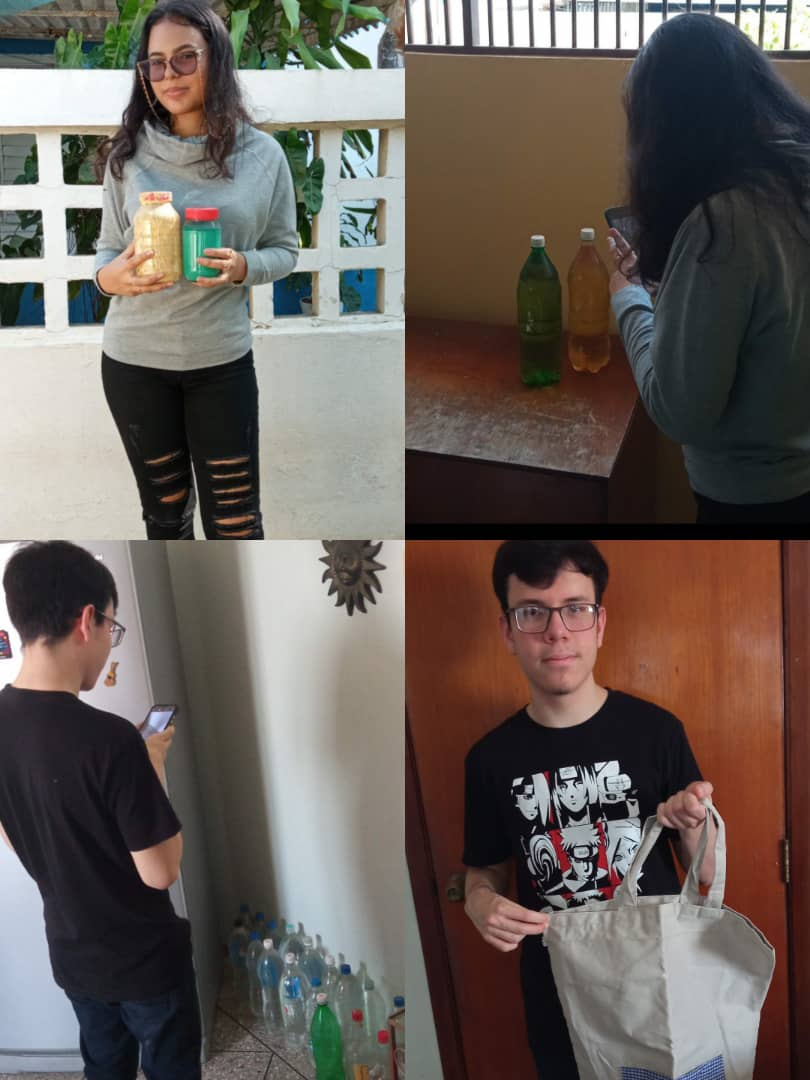
\includegraphics[width=10cm]{Media/Fotos/Foto 7 seguimiento.jpeg}
    \\\RaggedRight Fuente: Elaboración propia
    \label{fig:seguimiento}
\end{figure}

\newpage

Además, se emplearon listas de cotejo de 11 indicadores (Ver anexo 4) las cuales se rellenaron mensualmente por cada hogar que formó parte de la muestra seleccionada. Posteriormente, se hizo una lista de frecuencia para determinar la cantidad de veces con que se puso en práctica cada estrategia propuesta para la aplicación de las 3R de la ecología. 

\begin{table}[h!]
    \centering
    \captionsetup{singlelinecheck=false, justification=raggedright, labelsep=newline}
    \caption{\textit{Frecuencia de las estrategias propuestas para la aplicación de las 3R de la ecología}}
    \begin{tabular}{lcccc}
        \toprule
        Indicadores & Frecuencia & Porcentaje\\
        \midrule
        Se clasificó la basura & 3 & 13,64\% \\
        Se reutilizaron todo tipo de envases para almacenar objetos & 15 & 68,18\%\\
        Se reutilizaron desechos de tela para elaborar bolsas & 4 & 18,18\%\\
        Se utilizaron ambas caras del papel para reducir su desperdicio & 16 & 72,73\%\\
        Se emplearon servilletas de tela en lugar de las de papel & 3 & 13,64\%\\ 
        Se evitó el uso de platos, cucharas y vasos desechables & 18 & 81,82\%\\
        Se evitó comprar artículos empaquetados con bastante plástico & 0 & 0\%\\
        Se guardó en el congelador desechos animales & 9 & 40,91\%\\
        Se realizó un compost con desechos orgánicos & 10 & 45,45\%\\
        Se usaron botellas plásticas como macetas para plantas & 1 & 4,55\%\\
        Otros & 7 & 31,82\%\\
        \bottomrule\\
    \end{tabular}
    \\\RaggedRight Fuente: Elaboración propia
    \label{table:cuadro15}
\end{table}

Con la información suministrada se pudo observar que la medida aplicada con mayor frecuencia es evitar el uso de platos, cucharas y vasos desechables con un 81,82\%. Seguido a lo antes planteado, la segunda más empleada obtuvo un porcentaje de 72,73\% de las respuestas que corresponde al empleo de ambas caras del papel para reducir su desperdicio. Así mismo, se observó que hay un 68,18\% de la muestra analizada que reutilizaron envases para almacenar objetos. También, existe un porcentaje de los habitantes del 45,45\% que realizó un compost con desechos orgánicos. En menor medida, se pudo observar que se guardaron desechos animales en el congelador, la aplicación de otras estrategias y la reutilización de desechos de tela para elaborar bolsas, con un porcentaje del 40,91\%, 31,82\% y 18,18\% respectivamente. Además, los datos arrojados reflejan que las medidas usadas con menor frecuencia fueron el empleo de servilletas de tela en lugar de las de papel con un 13,64\%, la clasificación de la basura con un 13,64\% y el uso de botellas plásticas como macetas para plantas con un 4,55\%. Por último, los habitantes no aplicaron la estrategia de evitar comprar artículos empaquetados con bastante plástico.

\begin{figure}[h]
    \centering
    \captionsetup{singlelinecheck=false, justification=raggedright, labelsep=newline}
    \caption{\textit{Gráfico de la frecuencia de las estrategias propuestas para la aplicación de las 3R de la ecología}}
    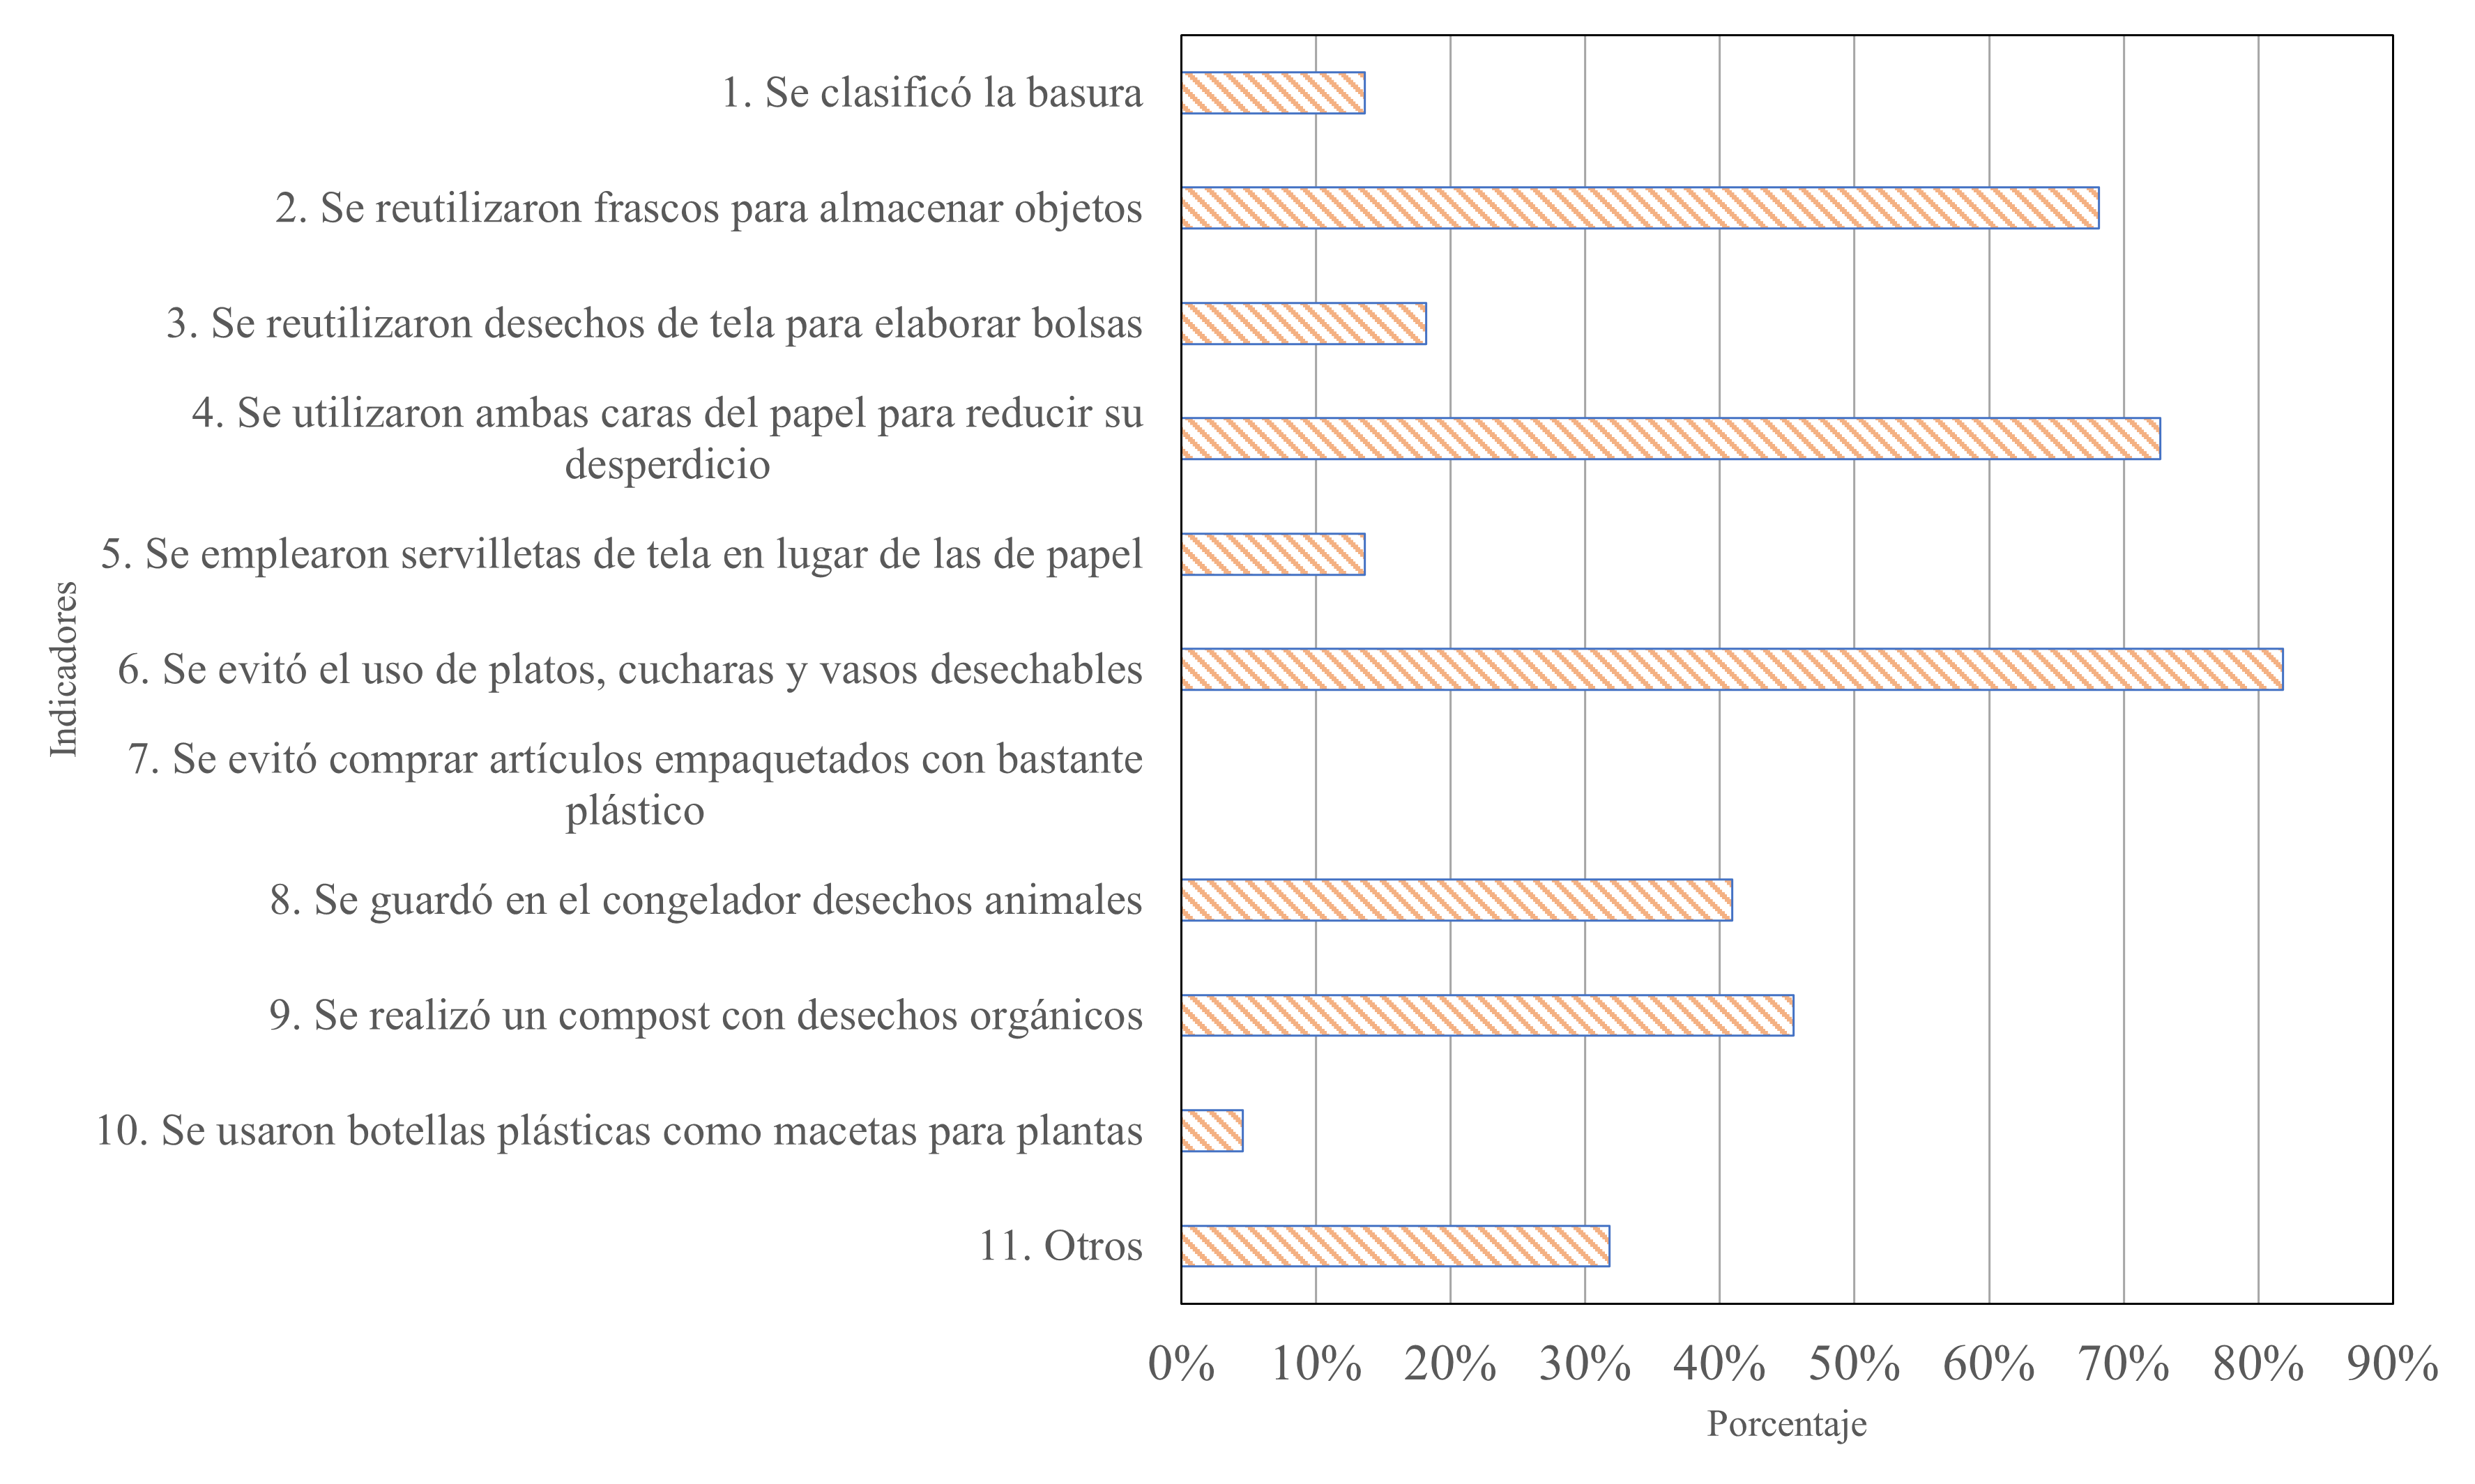
\includegraphics[width=15cm]{Media/Grafico Lista de Cotejo.png}
    \\\RaggedRight Fuente: Elaboración propia
    \label{fig:grafico}
\end{figure}

\newpage